\subsubsection{Digital Transmission Methods and Coding}
\label{ict:cns:henkel} \index{Henkel, Werner}

\paragraph{Research Team}
Werner Henkel (Professor), Fangning Hu (PhD Student), Neele von Deetzen (PhD
Student), Khaled Shawky Hassan (PhD Student), Apirath Limmanee (PhD Student)\\

We currently concentrate on iterative decoding and unequal error protection in
coding and physical transport. In iterative decoding, we study the convergence
behavior and properties of analog Turbo-like codes and the possible design of
Turbo and LDPC codes for unequal error protection (UEP). In the design of UEP
codes, we especially cooperate with ENSEA, France, and Lule\aa\ University,
Sweden. UEP is also the goal in our multicarrier research, where we design
bit-allocation algorithms that allow for easy realization of different
protection classes in an arbitrary way. UEP will be a must for current and
especially future triple-play data services to different devices at varying
channel qualities.

The analog codes have a strong relation to signal processing. Regarding
practical applications of such codes, we especially look into the correction
of impulse-noise and clipping effects. There, the most important task is to
determine statistical properties that allow for easy erasure marking, which
would support further decoding steps, analog and digital.

We further started a project on data transmission using ultrasound signals. We
currently design lab experiments to deliver data for later modeling of the
channel and disturbances.

%%% give a very short (150 words description of your research area)
%% Hint: this can be copied from the research areas document (../masterplan/research-areas)

\paragraph{Highlights}

The design of UEP Turbo codes by a pruning approach led us to a
structure that we named hybrid concatenation, a combination of outer
parallel and inner serial concatenation. The study of the decoding
convergence with so-called EXIT charts yielded the result that the
area between the curves describing the outer iterations depend on
the number of inner iterations. This allows for minimizing the
decoding complexity by a scheduling with varying number of
iterations in the different decoding steps
(Fig.~\ref{fig:henkel_1}). The pruning concept was also the starting
point for our design of UEP LDPC codes with an irregular check-node
profile (pat. pending).

\begin{figure}[ht]
  \centering
  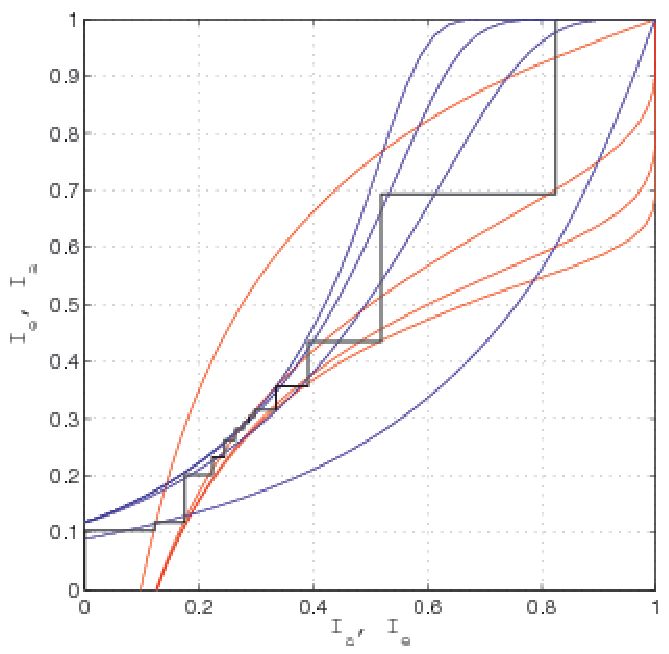
\includegraphics[width=7cm]{henkel_1}
 \caption{Convergence scheduling for hybrid concatenation}
%  \caption{Convergence scheduling for hybrid concatenation}
  \label{fig:henkel_1}
\end{figure}

In analog coding, we further improved the presentation of our proof that
Turbo-like decoding leads to a least-squares solution. We can now exactly
forecast the convergence limits for the stepsize and can also
modify it for every iteration to allow for very fast
convergence. For impulse-noise detection, we currently investigate new
statistical properties, e.g., the slope distribution, and correlation
approaches. This study will also close a gap in impulse-noise modeling
regarding the autocorrelation function of impulse noise.

By designing a new bit-allocation algorithm (pat. pending),
following the principles of an existing one by Chow, Cioffi, and
Bingham, we can obtain UEP properties in a very elegant way. It
allows for an arbitrary number of error-protection classes with
arbitrary margins between them and an arbitrary number of bits per
class. Fig.~\ref{fig:henkel_2} shows a resulting bit and power
allocation according to the channel SNRs, assuming three error
protection classes with a 3 dB separation.


\begin{figure}[ht]
  \centering
  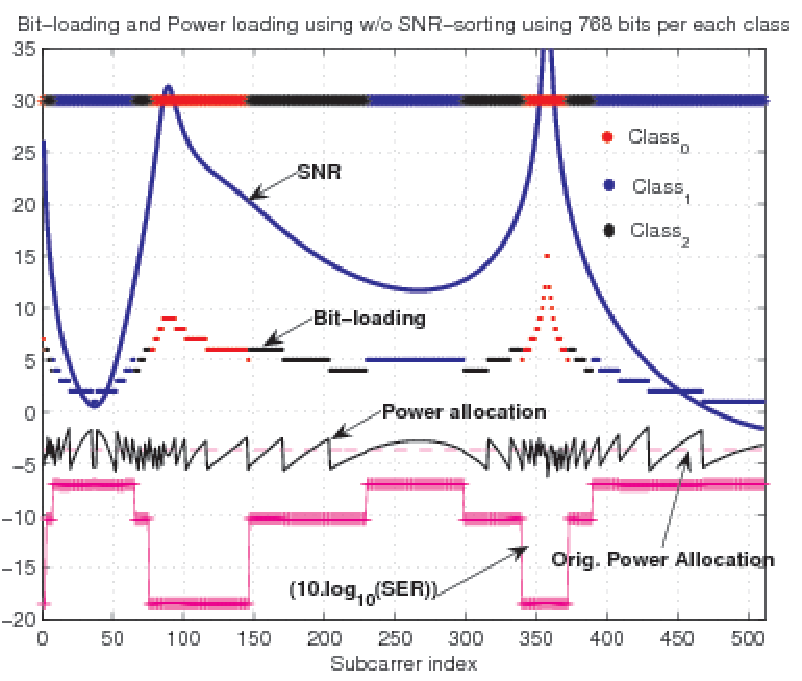
\includegraphics[width=7cm]{henkel_2}
  \caption{UEP bit and power allocation for three protection classes}
%  \caption{UEP bit and power allocation for three protection classes}
  \label{fig:henkel_2}
\end{figure}

\newpage
\paragraph{Organization}
% list the (research) events you have organized, if any,

\begin{enumerate}
\item Program Committee member of ICC 2006
\end{enumerate}

%\paragraph{Collaborations}
%\begin{enumerate}
%\item ...
%\item ...
%\item ...
%\end{enumerate}

\paragraph{Grants}
% list the running grants in 2005, if none have been received, please delete this
% subsection.
\begin{enumerate}
\item Funded by EU-IST STREP (FP 6), \emph{M-Pipe},  October 2004
- March 2007
\end{enumerate}

\paragraph{Patents}
\begin{enumerate}
\item  L. Sassatelli, W. Henkel, and D. Declercq. Check-Irregular LDPC Codes, Jan. 27
  2006. European Patent Application 06 100 979.1.
\item W. Henkel and K. Hassan. Unequal Error Protection Bit Loading for Multi-Carrier
  Transmission, Aug 30 2006. European Patent Application 06 119 771.1.
\end{enumerate}


%\paragraph{Publications}
% list the publications of 2005 (also accepted and in press), if none have been received, plese delete this
% subsection. Enter the publications into the SES publications database at
% http://kwarc.eecs.iu-bremen.de/ses-pubs/index.php and only reference them here.

%\begin{description}

%\item[Conference Proceedings]
  \nocite{Henkel_vDeetzen_IZS}
  \nocite{Hu_Henkel_Turbo}
  \nocite{Sassatelli_Henkel_Declercq_Turbo}
  \nocite{vDeetzen_Henkel_ISIT}
  \nocite{Henkel_Hassan_OFDM}
  \nocite{vDeetzen_ITG}
  \nocite{Hassan_Henkel_ITG}
%\item[Patents]
%  \nocite{Sassatelli_Henkel_Declercq_EP}
%  \nocite{Henkel_Hassan_EP}
%\end{description}

%%% Local Variables:
%%% mode: latex
%%% TeX-master: "report"
%%% End:
